% ថ្នាក់ទី ១១ (វិទ្យាសាស្ត្រ) · ជំពូកទី ៣ · មេរៀនទី ៣ · សៀវភៅទំព័រ ១២០–១២៧
\chapter{អនុគមន៍ច្រាសនៃអនុគមន៍ត្រីកោណមាត្រ}

\section{សេចក្តីផ្តើម}

អនុគមន៍ច្រាសនៃអនុគមន៍ត្រីកោណមាត្រ ត្រូវបានកំណត់យ៉ាងសាមញ្ញថាជាអនុគមន៍ច្រាសនៃអនុគមន៍ត្រីកោណមាត្ររបស់អនុគមន៍ស៊ីនុស កូស៊ីនុស តង់សង់ កូតង់សង់ ។ អនុគមន៍ច្រាសទាំងនេះត្រូវបានប្រើជាមួយមុំមួយចំនួននៃផលធៀបត្រីកោណមាត្រណាមួយ ។ អនុគមន៍ច្រាសនៃអនុគមន៍ត្រីកោណមាត្រត្រូវបានអនុវត្តន៍យ៉ាងសំខាន់ក្នុងវិស័យវិស្វកម្ម រូបវិទ្យា ធរណីមាត្រ និងការរុករក ។

\section{អនុគមន៍ច្រាសនៃអនុគមន៍ត្រីកោណមាត្រ}

យើងបានសិក្សាអនុគមន៍ត្រីកោណមាត្រនៅមេរៀនមុនរួចរាល់ហើយអំពី $\sin x$, $\cos x$ និង $\tan x$ ដែលត្រូវបានប្រើដើម្បីរកប្រវែងជ្រុងមួយមិនស្គាល់នៃត្រីកោណកែង ប្រសិនបើប្រវែងជ្រុងមួយ និងរង្វាស់មុំមួយត្រូវបានគេស្គាល់ ។

គេតាងអនុគមន៍ច្រាសនៃអនុគមន៍ត្រីកោណមាត្រតាមក្បួនដូចខាងក្រោម ៖
\begin{formulaBox}[និយមន័យ]
បើ $a = f(b)$ នោះអនុគមន៍ច្រាសគឺ $b = f^{-1}(a)$ ។
\end{formulaBox}

ដូច្នេះអនុគមន៍ច្រាសនៃអនុគមន៍ត្រីកោណមាត្រនៃ $\sin x$, $\cos x$ និង $\tan x$ ត្រូវបានកំណត់ដោយ $\sin^{-1}(x)$, $\cos^{-1}(x)$ និង $\tan^{-1}(x)$ ឬតាងដោយ $\arcsin(x)$, $\arccos(x)$ និង $\arctan(x)$ ។ អនុគមន៍ច្រាសនេះ ត្រូវបានប្រើដើម្បីរករង្វាស់មុំមិនស្គាល់នៃត្រីកោណកែងមួយ នៅពេលដែលប្រវែងជ្រុងពីរទៀតមិនស្គាល់ ។

\begin{example}[ឧទាហរណ៍]
បាតនៃជណ្តើរមួយ ត្រូវបានដាក់នៅចម្ងាយ $3$ ម៉ែត្រ ពីជញ្ជាំងកម្ពស់ $10$ ម៉ែត្រ និងផ្នែកខាងលើនៃជណ្តើរប៉ះនឹងកំពូលនៃជញ្ជាំង ។ តើរង្វាស់មុំដែលបង្កើតឡើងដោយជណ្តើរ និងដីមានរង្វាស់ស្មើនឹងប៉ុន្មានដឺក្រេ?
\begin{center}
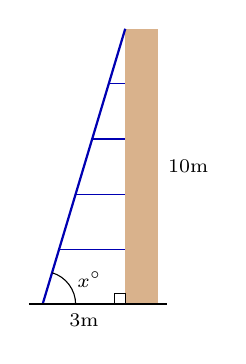
\begin{tikzpicture}[scale=0.35]
  \fill[brown!60] (3,0) rectangle (4.2,10);
  \draw[thick,blue!70!black] (0,0) -- (3,10);
  \draw[thick] (-0.5,0) -- (4.5,0);
  \draw (3,0) rectangle (2.6,0.4);
  \draw (1.2,0) arc (0:73:1.2); \node at (1.7,0.9) {\scriptsize $x^\circ$};
  \node[below] at (1.5,0) {\scriptsize $3$m}; \node[right] at (4.2,5) {\scriptsize $10$m};
  \foreach \t in {0.2,0.4,0.6,0.8} \draw[blue!70!black] ({3*\t},{10*\t}) -- (3,{10*\t});
\end{tikzpicture}
\end{center}
នៅទីនេះយើងមានត្រីកោណកែងមួយ ដែលយើងដឹងពីប្រវែងជ្រុងទាំងពីរ ពោលគឺ ជ្រុងទល់មុខ និងជ្រុងនៅជាប់នឹងមុំ ។ ដូច្នេះ យើងប្រើអនុគមន៍ច្រាសនៃអនុគមន៍តង់សង់ ។ ប្រសិនបើអ្នកបញ្ចូលវាទៅក្នុងម៉ាស៊ីនគិតលេខដែលគិតជា ``ដឺក្រេ'' នោះយើងបាន $\tan^{-1}\left(\dfrac{10}{3}\right) \approx 73.3^\circ$ ។ ប្រសិនបើអ្នកបានកំណត់ម៉ាស៊ីនគិតលេខទៅជារបៀបរ៉ាដ្យង់ អ្នកនឹងទទួលបាន $\tan^{-1}\left(\dfrac{10}{3}\right) \approx 1.28$ rd ។
\end{example}

ប្រសិនបើប្រើផលធៀបជ្រុងរបស់ត្រីកោណដែលមានមុំ $(45^\circ, 45^\circ, 90^\circ)$ និង $(30^\circ, 60^\circ, 90^\circ)$ នោះគេអាចរកឃើញតម្លៃមួយចំនួននៃអនុគមន៍ច្រាសត្រីកោណមាត្របានដោយមិនប្រើម៉ាស៊ីនគិតលេខ ។

\begin{example}[លំហាត់គំរូ ១]
រកតម្លៃនៃ $\cos^{-1}\left(\dfrac{\sqrt{3}}{2}\right)$ ។
\end{example}
\ans
អ្នកអាចចាំថានៅក្នុងត្រីកោណដែលមានមុំ $(30^\circ, 60^\circ, 90^\circ)$ ប្រសិនបើអ៊ីប៉ូតេនុសមានប្រវែងស្មើនឹង $1$ នោះជ្រុងវែងមានប្រវែង $\dfrac{\sqrt{3}}{2}$ ។ ដោយសារកូស៊ីនុសគឺជាសមាមាត្រនៃផ្នែកដែលនៅជាប់នឹងអ៊ីប៉ូតេនុស នោះតម្លៃច្រាសនៃកូស៊ីនុសគឺមុំ $30^\circ$ ឬប្រហែល $0.52$ រ៉ាដ្យង់ ។
\begin{center}
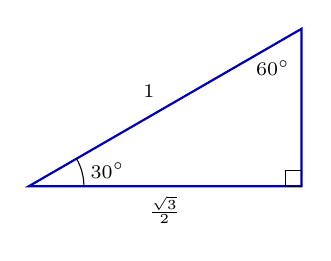
\begin{tikzpicture}[scale=2]
  \draw[thick,blue!70!black] (0,0) -- (1.732,0) -- (1.732,1) -- cycle;
  \draw (1.632,0) rectangle (1.732,0.1);
  \draw (0.35,0) arc (0:30:0.35); \node at (0.5,0.1) {\scriptsize $30^\circ$};
  \node at (1.55,0.75) {\scriptsize $60^\circ$};
  \node[above left] at (0.86,0.5) {\scriptsize $1$}; \node[below] at (0.86,0) {\scriptsize $\frac{\sqrt{3}}{2}$};
\end{tikzpicture}
\end{center}

\begin{note}[ចូរប្រយ័ត្ន]
ចំពោះអនុគមន៍ច្រាសនៃអនុគមន៍ត្រីកោណមាត្រ $\sin^{-1}x \ne \dfrac{1}{\sin x}$, $\cos^{-1}x \ne \dfrac{1}{\cos x}$ និង $\tan^{-1}x \ne \dfrac{1}{\tan x}$ ។
\end{note}

\begin{pro}
រកតម្លៃមុំដូចខាងក្រោម ៖
\begin{enumerate}[a]
  \item ចំពោះត្រីកោណកែង $ABC$ គេឱ្យជ្រុងមុំកែង $AB = 65$, $BC = 35$ ។ រកមុំ $\alpha$ នៃជ្រុង $AB$ និង $AC$ ។
  \item ចំពោះត្រីកោណកែង $LMN$ គេឱ្យជ្រុងមុំកែង $LM = 6$, $MN = 4$ ។ រកមុំ $\alpha$ នៃជ្រុង $LM$ និង $LN$ ។
  \item ចំពោះត្រីកោណកែង $PQR$ គេឱ្យជ្រុងមុំកែង $QR = 8$ និងអ៊ីប៉ូតេនុស $PR = 10$ ។ រកមុំ $\alpha$ នៃជ្រុង $PQ$ និង $PR$ ។
\end{enumerate}
\ans
ក. $\alpha \approx 28.30^\circ$ \qquad ខ. $\alpha \approx 33.69^\circ$ \qquad គ. $\alpha \approx 53.13^\circ$ ។
\end{pro}

\section{រូបមន្តអនុគមន៍ច្រាសនៃអនុគមន៍ត្រីកោណមាត្រ}

ខាងក្រោមជារូបមន្តគ្រឹះនៃអនុគមន៍ច្រាសនៃអនុគមន៍ត្រីកោណមាត្រ
\[
\begin{array}{|c|l|}\hline
\text{អនុគមន៍ច្រាស} & \text{រូបមន្ត}\\ \hline
\arcsin(x) & \sin^{-1}(-x) = -\sin^{-1}(x), \ x \in [-1, 1]\\ \hline
\arccos(x) & \cos^{-1}(-x) = \pi - \cos^{-1}(x), \ x \in [-1, 1]\\ \hline
\arctan(x) & \tan^{-1}(-x) = -\tan^{-1}(x), \ x \in \mathbb{R}\\ \hline
\text{arccot}(x) & \cot^{-1}(-x) = \pi - \cot^{-1}(x), \ x \in \mathbb{R}\\ \hline
\end{array}
\]

\section{ក្រាបនៃអនុគមន៍ច្រាសនៃអនុគមន៍ត្រីកោណមាត្រ}

ក្រាបនៃអនុគមន៍ច្រាសរបស់អនុគមន៍ត្រីកោណមាត្រ អាចបានពីក្រាបនៃអនុគមន៍ដើម ដោយការផ្លាស់ប្តូរអ័ក្ស $x$ និងអ័ក្ស $y$ ។ ប្រសិនបើ $(a, b)$ គឺជាចំណុចនៅលើក្រាបនៃអនុគមន៍ត្រីកោណមាត្រ បន្ទាប់មក $(b, a)$ ក្លាយជាចំណុចដែលត្រូវគ្នានៅលើក្រាបនៃអនុគមន៍ត្រីកោណមាត្រច្រាសរបស់វា ។ វាអាចត្រូវបានបង្ហាញថា ក្រាបនៃអនុគមន៍ច្រាសអាចបានពីក្រាបដែលត្រូវគ្នានៃអនុគមន៍ដើមជារូបភាពឆ្លុះគ្នាធៀបនឹងបន្ទាត់ $y = x$ ។

\subsection{ក្រាបនៃអនុគមន៍ \texorpdfstring{$y = \sin^{-1}(x)$}{y = arcsin x} ឬ \texorpdfstring{$y = \arcsin(x)$}{y = arcsin x}}

\begin{center}
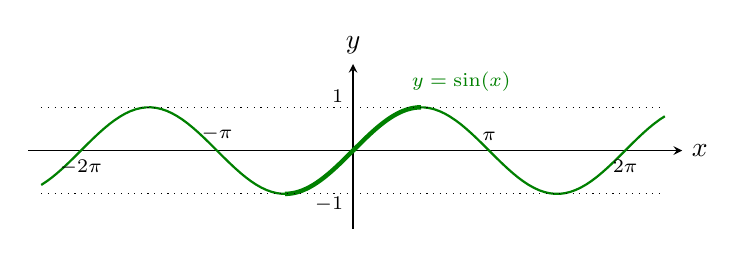
\begin{tikzpicture}[scale=0.55,>=stealth]
  \draw[->] (-7.5,0) -- (7.6,0) node[right] {$x$};
  \draw[->] (0,-1.8) -- (0,2) node[above] {$y$};
  \draw[green!50!black,thick,domain=-7.2:7.2,samples=120] plot (\x,{sin(\x r)});
  \draw[green!50!black,line width=1.6pt,domain=-1.5708:1.5708,samples=40] plot (\x,{sin(\x r)});
  \draw[dotted] (-7.2,1) -- (7.2,1); \draw[dotted] (-7.2,-1) -- (7.2,-1);
  \node[below] at (6.2832,0) {\scriptsize $2\pi$}; \node[below] at (-6.2832,0) {\scriptsize $-2\pi$};
  \node[above] at (3.1416,0) {\scriptsize $\pi$}; \node[above] at (-3.1416,0) {\scriptsize $-\pi$};
  \node[left] at (0,1.25) {\scriptsize $1$}; \node[left] at (0,-1.25) {\scriptsize $-1$};
  \node[green!50!black] at (2.5,1.6) {\scriptsize $y = \sin(x)$};
\end{tikzpicture}
\qquad
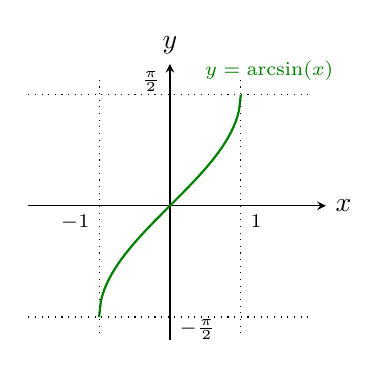
\begin{tikzpicture}[scale=0.9,>=stealth]
  \draw[->] (-2,0) -- (2.2,0) node[right] {$x$};
  \draw[->] (0,-1.9) -- (0,2) node[above] {$y$};
  \draw[green!50!black,thick,domain=-1:1,samples=80] plot (\x,{rad(asin(\x))});
  \draw[dotted] (-2,1.5708) -- (2,1.5708); \draw[dotted] (-2,-1.5708) -- (2,-1.5708);
  \draw[dotted] (-1,-1.8) -- (-1,1.8); \draw[dotted] (1,-1.8) -- (1,1.8);
  \node[below left] at (-1,0) {\scriptsize $-1$}; \node[below right] at (1,0) {\scriptsize $1$};
  \node[left] at (0,1.75) {\scriptsize $\frac{\pi}{2}$}; \node[right] at (0,-1.75) {\scriptsize $-\frac{\pi}{2}$};
  \node[green!50!black] at (1.4,1.9) {\scriptsize $y = \arcsin(x)$};
\end{tikzpicture}
\end{center}
\[
\begin{array}{|c|c|}\hline
\text{ដែនកំណត់នៃ } \sin x & \text{រ៉ង់}\\ \hline
-\frac{\pi}{2} \le x \le \frac{\pi}{2} & -1 \le y \le 1\\ \hline
\end{array}
\]
\[
\begin{array}{|c|c|}\hline
\text{ដែនកំណត់នៃ } \arcsin x & \text{រ៉ង់}\\ \hline
-1 \le x \le 1 & -\frac{\pi}{2} \le y \le \frac{\pi}{2}\\ \hline
\end{array}
\]

ប្រសិនបើយើងដាក់លក្ខខណ្ឌដែនកំណត់របស់ $f(x) = \sin(x)$ នៅចន្លោះ $\left[-\dfrac{\pi}{2}, \dfrac{\pi}{2}\right]$ នោះយើងបានវាជាអនុគមន៍មួយទល់មួយ ហើយរ៉ង់របស់វាគឺចន្លោះ $[-1, 1]$ ។ យើងកំណត់អនុគមន៍ច្រាសនៃ $f(x) = \sin(x)$ ដោយ $y = \sin^{-1}(x)$ ។ គេអានថា $y$ បញ្ច្រាសស៊ីនុស $x$ ហើយមានន័យថា $y$ ជាមុំចំនួនពិតដែលតម្លៃស៊ីនុសគឺ $x$ ។ សូមប្រយ័ត្នចំពោះសញ្ញាដែលបានប្រើ ។ សញ្ញា $(-1)$ មិនមែនជាស្វ័យគុណទេ មានន័យថា $\sin^{-1}x \ne \dfrac{1}{\sin x}$ ។ ដើម្បីជៀសវាងការសម្គាល់នេះ សៀវភៅខ្លះប្រើសញ្ញាណ $y = \arcsin(x)$ ជំនួសវិញ ។

គេឃើញថាក្រាបនៃអនុគមន៍ច្រាសនៃអនុគមន៍ស៊ីនុស ឆ្លុះគ្នាធៀបនឹងបន្ទាត់ $y = x$ នៃអនុគមន៍ស៊ីនុស ។

សូមកត់សម្គាល់ថា ដែនកំណត់ឥឡូវវាជារ៉ង់ ហើយរ៉ង់ឥឡូវវាជាដែនកំណត់ ។ ដោយសារដែនកំណត់ត្រូវបានដាក់លក្ខខណ្ឌ នោះមុំមានតម្លៃវិជ្ជមានគឺស្ថិតក្នុងកាដ្រង់ទី $1$ ហើយមុំតម្លៃអវិជ្ជមានស្ថិតនៅក្នុងកាដ្រង់ទី $4$ ។ ស្រដៀងគ្នានេះដែរ យើងអាចដាក់លក្ខខណ្ឌដែនកំណត់នៃអនុគមន៍កូស៊ីនុស និងតង់សង់ ដើម្បីធ្វើឱ្យវាជាអនុគមន៍មួយទល់មួយ ។

\subsection{ក្រាបនៃអនុគមន៍ \texorpdfstring{$y = \cos^{-1}(x)$}{y = arccos x} ឬ \texorpdfstring{$y = \arccos(x)$}{y = arccos x}}

\begin{center}
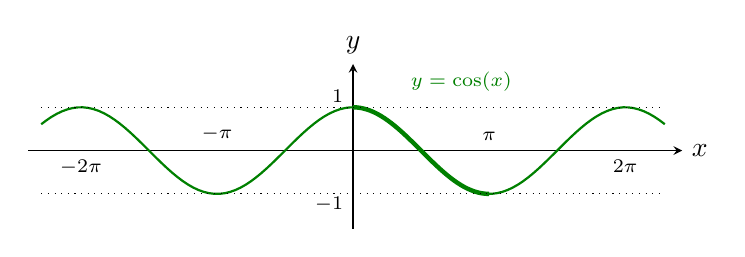
\begin{tikzpicture}[scale=0.55,>=stealth]
  \draw[->] (-7.5,0) -- (7.6,0) node[right] {$x$};
  \draw[->] (0,-1.8) -- (0,2) node[above] {$y$};
  \draw[green!50!black,thick,domain=-7.2:7.2,samples=120] plot (\x,{cos(\x r)});
  \draw[green!50!black,line width=1.6pt,domain=0:3.1416,samples=40] plot (\x,{cos(\x r)});
  \draw[dotted] (-7.2,1) -- (7.2,1); \draw[dotted] (-7.2,-1) -- (7.2,-1);
  \node[below] at (6.2832,0) {\scriptsize $2\pi$}; \node[below] at (-6.2832,0) {\scriptsize $-2\pi$};
  \node[above] at (3.1416,0) {\scriptsize $\pi$}; \node[above] at (-3.1416,0) {\scriptsize $-\pi$};
  \node[left] at (0,1.25) {\scriptsize $1$}; \node[left] at (0,-1.25) {\scriptsize $-1$};
  \node[green!50!black] at (2.5,1.6) {\scriptsize $y = \cos(x)$};
\end{tikzpicture}
\qquad
\begin{tikzpicture}[scale=0.8,>=stealth]
  \draw[->] (-2,0) -- (2.2,0) node[right] {$x$};
  \draw[->] (0,-0.5) -- (0,3.6) node[above] {$y$};
  \draw[green!50!black,thick,domain=-1:1,samples=80] plot (\x,{rad(acos(\x))});
  \draw[dotted] (-2,3.1416) -- (2,3.1416);
  \draw[dotted] (-1,0) -- (-1,3.3); \draw[dotted] (1,0) -- (1,3.3);
  \node[below] at (-1,0) {\scriptsize $-1$}; \node[below] at (1,0) {\scriptsize $1$};
  \node[left] at (0,3.35) {\scriptsize $\pi$}; \node[below left] at (0,0) {\scriptsize $0$};
  \node[green!50!black] at (-1.4,3.5) {\scriptsize $y = \arccos(x)$};
\end{tikzpicture}
\end{center}
\[
\begin{array}{|c|c|}\hline
\text{ដែនកំណត់នៃ } \cos x & \text{រ៉ង់}\\ \hline
0 \le x \le \pi & -1 \le y \le 1\\ \hline
\end{array}
\]
\[
\begin{array}{|c|c|}\hline
\text{ដែនកំណត់នៃ } \arccos x & \text{រ៉ង់}\\ \hline
-1 \le x \le 1 & 0 \le y \le \pi\\ \hline
\end{array}
\]
ដែនកំណត់នៃអនុគមន៍ច្រាសនៃអនុគមន៍កូស៊ីនុសគឺ $[-1, 1]$ ហើយរ៉ង់គឺ $[0, \pi]$ ។ នោះមានន័យថាមុំមានតម្លៃវិជ្ជមានស្ថិតនៅក្នុងកាដ្រង់ទី $1$ ហើយមុំមានតម្លៃអវិជ្ជមានស្ថិតក្នុងកាដ្រង់ទី $2$ ។

\subsection{ក្រាបនៃអនុគមន៍ \texorpdfstring{$y = \tan^{-1}(x)$}{y = arctan x} ឬ \texorpdfstring{$y = \arctan(x)$}{y = arctan x}}

\begin{center}
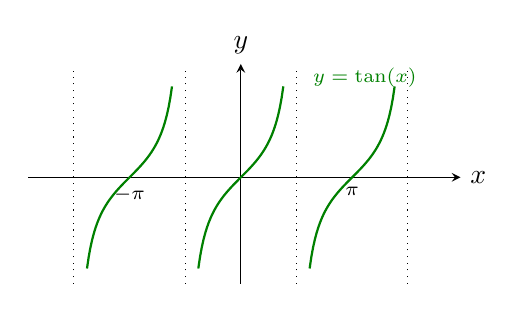
\begin{tikzpicture}[scale=0.45,>=stealth]
  \draw[->] (-6,0) -- (6.2,0) node[right] {$x$};
  \draw[->] (0,-3) -- (0,3.2) node[above] {$y$};
  \foreach \c in {-3.1416,0,3.1416} \draw[green!50!black,thick,domain=\c-1.2:\c+1.2,samples=50] plot (\x,{tan((\x-\c) r)});
  \foreach \a in {-4.7124,-1.5708,1.5708,4.7124} \draw[dotted] (\a,-3) -- (\a,3);
  \node[below] at (3.1416,0) {\scriptsize $\pi$}; \node[below] at (-3.1416,0) {\scriptsize $-\pi$};
  \node[green!50!black] at (3.5,2.8) {\scriptsize $y = \tan(x)$};
\end{tikzpicture}
\qquad
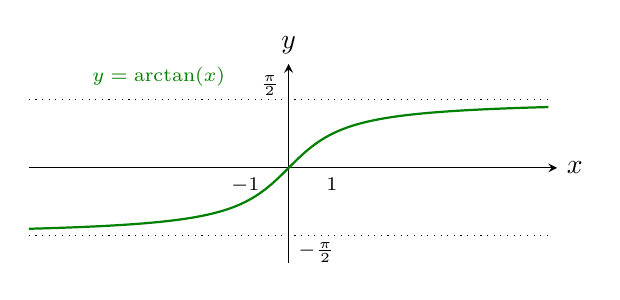
\begin{tikzpicture}[scale=0.55,>=stealth]
  \draw[->] (-6,0) -- (6.2,0) node[right] {$x$};
  \draw[->] (0,-2.2) -- (0,2.4) node[above] {$y$};
  \draw[green!50!black,thick,domain=-6:6,samples=80] plot (\x,{rad(atan(\x))});
  \draw[dotted] (-6,1.5708) -- (6,1.5708); \draw[dotted] (-6,-1.5708) -- (6,-1.5708);
  \node[left] at (0,1.9) {\scriptsize $\frac{\pi}{2}$}; \node[right] at (0,-1.95) {\scriptsize $-\frac{\pi}{2}$};
  \node[below] at (-1,0) {\scriptsize $-1$}; \node[below] at (1,0) {\scriptsize $1$};
  \node[green!50!black] at (-3,2.1) {\scriptsize $y = \arctan(x)$};
\end{tikzpicture}
\end{center}
\[
\begin{array}{|c|c|}\hline
\text{ដែនកំណត់នៃ } \tan x & \text{រ៉ង់}\\ \hline
\left(-\frac{\pi}{2}, \frac{\pi}{2}\right) & (-\infty, +\infty)\\ \hline
\end{array}
\]
\[
\begin{array}{|c|c|}\hline
\text{ដែនកំណត់នៃ } \arctan x & \text{រ៉ង់}\\ \hline
(-\infty, +\infty) & \left(-\frac{\pi}{2}, \frac{\pi}{2}\right)\\ \hline
\end{array}
\]
ដែនកំណត់អនុគមន៍ច្រាសនៃអនុគមន៍តង់សង់គឺ $(-\infty, +\infty)$ ហើយរ៉ង់គឺ $\left(-\dfrac{\pi}{2}, \dfrac{\pi}{2}\right)$ ។ អនុគមន៍ច្រាសនៃអនុគមន៍តង់សង់មានតម្លៃក្នុងកាដ្រង់ទី $1$ និងទី $4$ ។ ដំណើរការដូចគ្នានេះត្រូវបានប្រើដើម្បីស្វែងរកអនុគមន៍ច្រាសសម្រាប់អនុគមន៍ត្រីកោណមាត្រដែលនៅសេសសល់ ដូចជាអនុគមន៍កូតង់សង់ជាដើម ។ល។

\section{តារាងអនុគមន៍ច្រាសនៃអនុគមន៍ត្រីកោណមាត្រ}

\[
\renewcommand{\arraystretch}{1.5}
\begin{array}{|c|c|c|}\hline
\text{អនុគមន៍} & \text{ដែនកំណត់} & \text{រ៉ង់}\\ \hline
\sin^{-1}(x) & [-1, 1] & \left[-\frac{\pi}{2}, \frac{\pi}{2}\right]\\ \hline
\cos^{-1}(x) & [-1, 1] & [0, \pi]\\ \hline
\tan^{-1}(x) & (-\infty, +\infty) & \left(-\frac{\pi}{2}, \frac{\pi}{2}\right)\\ \hline
\cot^{-1}(x) & (-\infty, +\infty) & (0, \pi)\\ \hline
\end{array}
\]

\begin{example}[លំហាត់គំរូ ២]
រកតម្លៃនៃ $\cos^{-1}\left(-\dfrac{1}{2}\right)$ ។
\end{example}
\ans
តាង $x = \cos^{-1}\left(-\dfrac{1}{2}\right)$ នាំឱ្យ $\cos x = -\dfrac{1}{2}$ ។ ដោយរ៉ង់នៃ $\cos^{-1}x$ គឺ $[0, \pi]$ នោះយើងបានតម្លៃ $\cos^{-1}\left(-\dfrac{1}{2}\right) = \dfrac{2\pi}{3}$ ។

\begin{pro}
\begin{enumerate}[a]
  \item រកតម្លៃមុំនៃ $\cos^{-1}\left(\dfrac{\sqrt{3}}{2}\right)$
  \item រកតម្លៃមុំនៃ $\tan^{-1}(1) + \cos^{-1}\left(-\dfrac{1}{2}\right) + \sin^{-1}\left(-\dfrac{1}{2}\right)$
  \item រកតម្លៃមុំនៃ $\tan^{-1}(\sqrt{3}) - \cot^{-1}(-\sqrt{3})$ ។
\end{enumerate}
\ans
ក. $\dfrac{\pi}{6}$ \qquad ខ. $\dfrac{3\pi}{4}$ \qquad គ. $-\dfrac{\pi}{2}$ ។
\end{pro}

\section{លក្ខណៈអនុគមន៍ច្រាសនៃអនុគមន៍ត្រីកោណមាត្រ}

\begin{formulaBox}[លក្ខណៈ]
\begin{itemize}
  \item $\sin^{-1}(\sin x) = x$ ចំពោះ $-\dfrac{\pi}{2} \le x \le \dfrac{\pi}{2}$
  \item $\cos^{-1}(\cos x) = x$ ចំពោះ $0 \le x \le \pi$
  \item $\tan^{-1}(\tan x) = x$ ចំពោះ $-\dfrac{\pi}{2} < x < \dfrac{\pi}{2}$
  \item $\sin(\sin^{-1}x) = x$ ចំពោះ $-1 \le x \le 1$
  \item $\cos(\cos^{-1}x) = x$ ចំពោះ $-1 \le x \le 1$
  \item $\tan(\tan^{-1}x) = x$ ចំពោះ $x \in \mathbb{R}$
  \item $\cot^{-1}(\cot x) = x$ ចំពោះ $x \in (0, \pi)$
\end{itemize}
\end{formulaBox}

\begin{example}[ឧទាហរណ៍]
\begin{enumerate}[a]
  \item $\sin(\sin^{-1}0.5) = 0.5$, \ $\sin(\sin^{-1}1.5) \ne 1.5$ ព្រោះ $-1 \le x \le 1$
  \item $\sin^{-1}[\sin(-1.5)] = -1.5$, \ $\sin^{-1}[\sin(-2)] \ne -2$ ព្រោះ $-\dfrac{\pi}{2} \le x \le \dfrac{\pi}{2}$ ។
\end{enumerate}
\end{example}

\textbf{\textcolor{blue!60!black}{☞ ការគណនាដោយមិនចាំបាច់ប្រើម៉ាស៊ីនគិតលេខ}}

\begin{example}[លំហាត់គំរូ ៣]
រកតម្លៃនៃ $\sin^{-1}\left(-\dfrac{1}{2}\right)$ ។
\end{example}
\ans
តាង $y = \sin^{-1}\left(-\dfrac{1}{2}\right)$ \ $\sin y = \sin\left(\sin^{-1}\left(-\dfrac{1}{2}\right)\right)$ នោះ $\sin y = -\dfrac{1}{2}$ ដែល $-\dfrac{\pi}{2} \le y \le \dfrac{\pi}{2}$ តាមតារាងត្រីកោណមាត្រយើងបាន $y = -\dfrac{\pi}{6} = \sin^{-1}\left(-\dfrac{1}{2}\right)$ ទោះបីជា $\sin\left(\dfrac{11\pi}{6}\right) = -\dfrac{1}{2}$ ក៏វាមិនមែនជាចម្លើយដែរ ព្រោះ $y$ នៅក្នុងចន្លោះ $\left[-\dfrac{\pi}{2}, \dfrac{\pi}{2}\right]$ ។ ដូច្នេះ $\sin^{-1}\left(-\dfrac{1}{2}\right) = -\dfrac{\pi}{6}$ ។

\textbf{\textcolor{blue!60!black}{☞ ការគណនាដោយប្រើម៉ាស៊ីនគិតលេខ}}
\begin{itemize}
  \item មានប្រភេទម៉ាកផ្សេងៗគ្នានៅលើម៉ាស៊ីនគិតលេខ ដូច្នេះសូមអានការណែនាំនៅក្នុងសៀវភៅណែនាំរបស់អ្នកប្រើប្រាស់ ។
  \item ត្រូវប្រាកដថាកំណត់ម៉ាស៊ីនគិតលេខនៅលើទម្រង់រ៉ាដ្យង់ ។
  \item ប្រសិនបើម៉ាស៊ីនគិតលេខបង្ហាញកំហុស នោះតម្លៃឬលេខដែលប្រើមិនស្ថិតនៅក្នុងដែនកំណត់នៃអនុគមន៍ត្រីកោណមាត្រទេ ។
\end{itemize}

\begin{example}[ឧទាហរណ៍ ១]
បើអ្នកចុច $\sin^{-1}(1.548)$ នៅលើម៉ាស៊ីនគិតលេខរបស់អ្នកឧបករណ៍នឹងបញ្ជាក់ថាមានកំហុស គឺដោយសារតែ $1.548$ មិនស្ថិតនៅក្នុងដែនកំណត់នៃ $\sin^{-1}$ ទេ ។
\end{example}

\begin{example}[ឧទាហរណ៍ ២]
\begin{enumerate}[a]
  \item $\cos(\cos^{-1}0.5) = 0.5$
  \item $\cos(\cos^{-1}1.5) \ne 1.5$ ព្រោះ $-1 \le x \le 1$
  \item $\cos^{-1}[\cos(0.5)] = 0.5$
  \item $\cos^{-1}[\cos(-2)] \ne -2$ ព្រោះ $0 \le x \le \pi$ ។
\end{enumerate}
\end{example}

\textbf{\textcolor{blue!60!black}{☞ ការគណនាដោយមិនចាំបាច់ប្រើម៉ាស៊ីនគិតលេខ}}

\begin{example}[ឧទាហរណ៍]
រកតម្លៃនៃ $\cos(\cos^{-1}0.6)$ ដោយ $-1 < 0.6 < 1$ នោះ $\cos(\cos^{-1}0.6) = 0.6$ ។
\end{example}

\begin{example}[លំហាត់គំរូ ៤]
រកតម្លៃនៃ $\arccos\left(-\dfrac{1}{\sqrt{2}}\right)$ ។
\end{example}
\ans
$\arccos\left(-\dfrac{1}{\sqrt{2}}\right)$ គឺដូចគ្នាទៅនឹង $\cos y = -\dfrac{1}{\sqrt{2}}$ ដែល $0 < y < \pi$ ។ តាមតារាងត្រីកោណមាត្រនិងរង្វង់ត្រីកោណមាត្រ គេបាន $\dfrac{3\pi}{4}$ ជាចម្លើយ នោះគេបាន $y = \dfrac{3\pi}{4} = \arccos\left(-\dfrac{1}{\sqrt{2}}\right)$ ។

\textbf{\textcolor{blue!60!black}{☞ ការគណនាដោយប្រើម៉ាស៊ីនគិតលេខ}}

\begin{example}[ឧទាហរណ៍ ៣]
ប្រសិនបើអ្នកចុច $\cos^{-1}(1.238)$ នៅលើម៉ាស៊ីនគិតលេខរបស់អ្នកឧបករណ៍នឹងបញ្ជាក់ថាមានកំហុស គឺដោយសារតែ $1.238$ មិនស្ថិតនៅក្នុងដែនកំណត់នៃ $\cos^{-1}$ ទេ ។
\end{example}

\begin{example}[ឧទាហរណ៍ ៤]
\begin{enumerate}[a]
  \item $\tan(\tan^{-1}2) = 2$
  \item $\tan[\tan^{-1}(-1.5)] = -1.5$
  \item $\tan^{-1}[\tan(-0.5)] = -0.5$
  \item $\tan^{-1}[\tan(-2)] \ne -2$ ព្រោះ $-\dfrac{\pi}{2} < x < \dfrac{\pi}{2}$ ។
\end{enumerate}
\end{example}

\begin{example}[លំហាត់គំរូ ៥]
រកតម្លៃមុំនៃ $y = \tan^{-1}(\sqrt{3})$ ។
\end{example}
\ans
ដោយ $\tan^{-1}(\sqrt{3})$ ដូចគ្នាជាមួយនឹង $\tan y = \sqrt{3}$ ដែល $-\dfrac{\pi}{2} < y < \dfrac{\pi}{2}$ ។ ដូច្នេះ $y = \dfrac{\pi}{3} = \tan^{-1}(\sqrt{3})$ ។

\begin{example}[លំហាត់គំរូ ៦]
រកតម្លៃនៃ $\tan[\tan^{-1}(56)]$ ។
\end{example}
\ans
ដោយ $\tan(\tan^{-1}x) = x$ ដែល $-\infty < x < \infty$ នោះយើងបាន $\tan[\tan^{-1}(56)] = 56$ ។

\begin{pro}
\begin{enumerate}[a]
  \item រកតម្លៃនៃ $\cos^{-1}x$ ចំពោះ $x = \dfrac{\sqrt{3}}{2}$ ។
  \item រកតម្លៃ $\tan^{-1}\left(\sin\left(-\dfrac{\pi}{2}\right)\right)$ ។
  \item រកតម្លៃ $\cos^{-1}\left(\cos\left(\dfrac{13\pi}{6}\right)\right)$ ។
\end{enumerate}
\ans
ក. $\dfrac{\pi}{6}$ \qquad ខ. $-\dfrac{\pi}{4}$ \qquad គ. $\dfrac{\pi}{6}$ ។
\end{pro}

\section*{លំហាត់អនុវត្តន៍}
\begin{enumerate}[1]
  \item រកតម្លៃនៃ $\sin^{-1}\left(\sin\left(\dfrac{\pi}{6}\right)\right)$ ។
  \item រកតម្លៃ $\sin\left(\cos^{-1}\dfrac{3}{5}\right)$ ។
  \item រកតម្លៃ $\tan^{-1}\left(\tan\left(\dfrac{9\pi}{8}\right)\right)$ ។
  \item រកតម្លៃ $\tan(\tan^{-1}(-4))$ ។
  \item រកតម្លៃ $\sin^{-1}\left(\cos\left(\sin^{-1}\left(\dfrac{\sqrt{3}}{2}\right)\right)\right)$ ។
  \item បង្ហាញថា $\tan(\cot^{-1}x) = \cot(\tan^{-1}x)$ ។
  \item បង្ហាញថា $2\sin^{-1}\left(\dfrac{3}{5}\right) - \tan^{-1}\left(\dfrac{17}{31}\right) = \dfrac{\pi}{4}$ ។
  \item បង្ហាញថា $\cot^{-1}7 + \cot^{-1}8 + \cot^{-1}18 = \cot^{-1}3$ ។
  \item ប្រៀបធៀប $\tan^{-1}1$ និង $\tan 1$ ។
  \item រកតម្លៃនៃ $\sin\left(2\tan^{-1}\left(\dfrac{2}{3}\right)\right) + \cos(\tan^{-1}\sqrt{3})$ ។
  \item ដោះស្រាយសមីការ $\tan^{-1}\left\{\dfrac{1 - x}{1 + x}\right\} = \left(\dfrac{1}{2}\right)\tan^{-1}x$, $x > 0$ ។
  \item រកតម្លៃ $x$ ដែលផ្ទៀងផ្ទាត់សមីការ $\sin^{-1}x + \sin^{-1}(1 - x) = \cos^{-1}x$ ។
  \item ដោះស្រាយសមីការ $\sin^{-1}6x + \sin^{-1}6\sqrt{3}x = -\dfrac{\pi}{2}$ ។
\end{enumerate}
